\documentclass[11pt,a4paper]{report}
\usepackage[utf8x]{inputenc}
\usepackage[T1]{fontenc}
% only used to make the introduction page look nice
%\usepackage{gentium}
\usepackage{mathptmx} % Use Times Font
\usepackage{minted}
% Template taken very gladly from Robert Jones and expanded greatly for a third year project
\usepackage[
    backend=biber,
    style = numeric
    ]{biblatex}

% Fill out the location of your references
\addbibresource{SNAIL.bib}

%%%
\usepackage{soul}
\usepackage{amsmath}
\usepackage{float}
\usepackage{ragged2e}
\usepackage{xcolor}
\usepackage{mathtools}
\DeclarePairedDelimiter\bra{\langle}{\rvert}
\DeclarePairedDelimiter\ket{\lvert}{\rangle}
\DeclarePairedDelimiterX\braket[2]{\langle}{\rangle}{#1\,\delimsize\vert\,\mathopen{}#2}
\DeclarePairedDelimiterX\braketmid[3]{\langle}{\rangle}{#1\,\delimsize\vert\,#2 \vert\,\mathopen{}#3}

\usepackage[%
  bookmarks=false,
  colorlinks,
  linkcolor=blue,
  urlcolor=blue,
  citecolor=blue,
  plainpages=false,
  pdfpagelabels,
  final,
  breaklinks=true
]{hyperref}

\usepackage{multicol}

\usepackage[pdftex]{graphicx} % Required for including pictures
%\usepackage{calc} % To reset the counter in the document after title page
%\usepackage{enumitem} % Includes lists

\frenchspacing % No double spacing between sentences
\linespread{1.05} % Set linespace
\usepackage[a4paper, 
lmargin=0.15\paperwidth, rmargin=0.15\paperwidth, tmargin=0.1\paperheight, bmargin=0.12\paperheight]{geometry} %margins
\usepackage{fancyhdr} 
%\usepackage{parskip}

%\usepackage[all]{nowidow} % Tries to remove widows
\usepackage[protrusion=true,expansion=true]{microtype} 
\usepackage{titlesec} % This makes the chapter titles not have the annoying 'Chapter 1' header
\titleformat{\chapter}[display]
  {\normalfont\huge\bfseries}{}{0pt}{\Huge}

\date{}

\author{Alex Benitez}


\begin{document}

\begin{titlepage}
    \centering
    \vspace*{3cm} % Adjust vertical space at the top
    
    % Large Title
    {\LARGE\bfseries Calculating the Harmonic Response of Gas Particles Using the SFA Approximation \par}
    
    \vspace{0.5cm}
    
    % University Name
    {\Large King's College London \par}
    
    \vspace{0.5cm}
    
    % Course and Project Info
    {\large 6CCP3131 Third Year Project \par}
    
    \vspace{0.5cm}
    
    % Author's Name
    {\large \textbf{Alex Benitez} \par}
    
    \vspace{0.5cm}
    
    % Supervisor's Name
    {\large Supervisor: \textbf{Amelle Zaïr }\par}

    \vspace{2cm}
    {\small \textbf{Abstract:} Machine Learning for image recognition requires large datasets to be trained. High Harmonic Generation is a very computationally expensive process to simulate, inhibiting the ability to train Neural Networks without experimental data. This report outlines an Open-Source package called SNAIL, which greatly speeds up calculation of the HHG spectrum generated by various types of particles and customizable strong fields.}  %Modify before sending off
    
    
    \vfill % Push everything above to the center vertically
    \includegraphics[width=0.5\textwidth]{logosnail.png}
    
\end{titlepage}

% Bottom of the page
    %\includegraphics[width=4.19in]{SNAIL.jpg}\par\vspace{1cm}
\newpage
\tableofcontents
\newpage


\newgeometry{left=0.15\paperwidth, right=0.15\paperwidth, top=-0.065\paperheight, bottom=0.03\paperheight}

%\vspace{-20mm}
%\newgeometry{top=3cm, bottom=1.5cm, left=1.5cm, right=1.5cm}
\thispagestyle{fancy}
\setlength{\footskip}{0pt}
\chapter{Theoretical Background}
\vspace{-10mm}
\section{The Three Step Model}
Most nonlinear optical phenomena follow a simple relationship where the magnitude of the response drops linearly or exponentially with the order of the effect. In 1993 a series of experiments \cite{firstatto1}\cite{firstatto2} delivered a very surprising result, using high intensity lasers, a gas medium would generate a response with harmonics (pulses with multiples of the driving laser frequency) up to two orders of magnitude of the driving pulse, far exceeding any intuitive understanding. The simplest way to explain this result is with the three-step model, the origin of which is debated but generally attributed to \cite{threestep1}\cite{threestep2}\cite{threestep3}. In the model, a strong laser pulse deforms the potential well of an electron in an atom, the electron tunnels into the continuum at 0 velocity under the influence of the electric field, during a laser cycle it travels away and comes back to the atom, where it can scatter or recombine. Focusing only on the recombination, the electron will emit a pulse, equivalent to the kinetic energy gained in the continuum. This simple model allows for an intuitive understanding of most of the effects observed in High Harmonic Generation (HHG).
\\
\begin{figure}[h]

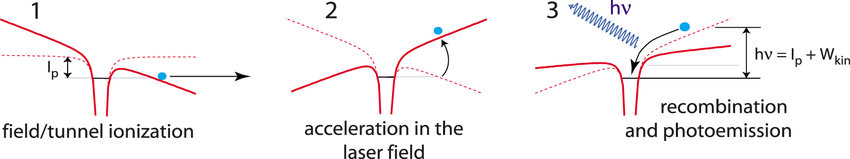
\includegraphics[width=1\textwidth]{threestep.jpg}
\caption{Graphic picturing the three step model of HHG, reprinted from \cite{Threestepfig}}
\end{figure}

Experimentally the maximum harmonic was found to be $I_p + 3U_p$ where $I_p$ is the ionization potential of the atom and $U_p = \frac{e^2 E^2}{4mw^{2}_o}$ is the ponderomotive energy, which is just the time averaged kinetic energy. Using the three step model, the maximum kinetic energy of the electron can be modelled, by considering a series of electrons under the influence of a simple laser the maximum kinetic energy is found to be around 3.17 $U_p$ which will have $I_p$ added to it as soon as the electron recombines, closely matching experimental results.

\begin{figure}[h]
\centering
\includegraphics[width=0.9\textwidth]{kineticplot.png}
\caption{Plot demonstrating the 1D trajectories of electrons released during positive electric field values. From top to bottom, the driving field, distance of the electron from the nucleus and the maximum kinetic energy at recombination. In the second plot the trajectory with the highest kinetic energy is black.}
\end{figure}
\newpage

\newgeometry{left=0.15\paperwidth, right=0.15\paperwidth, top=0.1\paperheight, bottom=0.12\paperheight}

\section{The Strong Field Approximation}
In 1994, Maciej Lewenstein and others introduced one of the most powerful tools to calculate HHG in a landmark paper \cite{lewensteinog}. The main assumptions of the Lewenstein model are: a) The ground state does not deplete, b) The ground state is the only bound state that affects the evolution of the system, c) The free electron only feels the external field, ignoring the atomic potential. For the ground state to not deplete, the ponderomotive force should be below $U_{sat}$, the saturation potential where all of the atoms ionize during interaction. Following the method set out in \cite{smirnovaMultielectronHighHarmonic2013}, \cite{propagators} and \cite{Emiliomasters}, for the remainder of the text except where explicitly stated we use atomic units. We start with the TDSE of one shell electron:

\begin{equation} 
	i\frac{\partial}{\partial t} \ket{\psi(t)} = \left[-\frac{1}{2} \nabla^2 + V(r) - Ecos(t)x\right] \ket{\psi(t)} = \hat{H}(t) \ket{\psi(t)}
	\label{TDSE}
\end{equation}
Here V(r) is the atomic potential, $Ecos(t)$ is the time-varying electric field from the driving pulse and $\hat{H}(t)$ is the Hamiltonian. What we want to find is the induced dipole, which is proportional to the response and given by:
\begin{equation}
\mathbf{D}(t) = \bra{\psi(t)}\hat{\mathbf{d}}\ket{\psi(t)}
\end{equation}
To calculate this, however, we need to represent the wavefunction in a convenient form; so we introduce propagators. A possible solution for \eqref{TDSE}, is:
\begin{equation}
\ket{\psi(t)} = e^{-i\int_{0}^{t} \hat{H}(t')dt'}\ket{\psi(0)} = e^{-i\int_{0}^{t} \hat{H}(t')dt'} \ket{g}
\end{equation}
Where we set the initial state of the wavefunction as $\ket{g}$ implying the electron starts in the ground state in the atomic well. However, this form is not actually useful; the Hamiltonian can be split into any two parts, which we choose as $\hat{H} = \hat{H}_0 + \hat{V}_L$. In this case $\hat{H}_0$ is the Hamiltonian of the atomic potential, and $\hat{V}_L$ is the interaction with the laser. To split it, we have to find an expression for the propagator of our full Hamiltonian, which we will call $U_1(t,t')$, first we assume:
\begin{equation}
i\frac{\partial}{\partial t}	U_0(t,t') = H_0 U_0(t,t') \qquad U_0(t,t) = 1
\end{equation}
and we want to solve:
\begin{equation}
i\frac{\partial}{\partial t}	U(t,t') = (H_0 + \Delta H)U(t,t') \qquad U(t,t) = 1
\end{equation}
The Dyson expansion states that this can be found recursively, and only taking the first term of the expansion since we neglect interaction with the atomic potential:
\begin{equation}
U(t,t') = U_0(t,t') \; -\; i\int^{t}_{t'} dt'' U(t,t'')\Delta H(t'') U_0(t'',t')
\end{equation}
A quick way to prove this is to substitute it in for itself which assumes knowledge of $U_0$ and U being a solution of itself and uses the Leibniz integral rule in the second line:
\begin{equation}
\begin{split}
i \frac{\partial U(t,t')}{\partial t} = i \frac{\partial}{\partial t} \left[-i \int^{t}_{t'} dt'' U(t,t'')\Delta H(t'') U_0(t'',t') + U_0)t,t')\right] \\
=U(t,t)\Delta H(t) U_0(t,t') + \int^{t}_{t'} dt'' i\frac{\partial U(t,t'')}{\partial t} \Delta H (t'') U_0(t'',t') + i\frac{\partial}{\partial t} U_0(t,t') \\
 = (H_0  + \Delta H) \int^{t}_{t'} dt'' U(t,t'')\Delta H (t'') U_0(t'',t') + \Delta H U_0(t,t') + H_0U_0(t,t') \\
= (H_0 + \Delta H )U(t,t')
\end{split}
\end{equation}

Finally, substituting in back for the exponential terms, the wavefunction can be expressed as:
\begin{equation}
\ket{\psi(t)} = e^{-i\int_{0}^{t} \hat{H}_0(t'')dt''}\ket{g} \; -\; i\int^{t}_{0}dt' \left[e^{-i\int_{t'}^{t} \hat{H}(t'')dt''}\right]\hat{V}_L(t')\left[e^{-i\int_{0}^{t'} \hat{H}_0(t'')dt''}\right]\ket{g}
	\label{propagatorfull}
\end{equation}
This very scary equation is surprisingly intuitive, the first standalone exponential term is the evolution of the non-ionized part of the electronic wavefunction. Inside the integral, the first exponential term acting on the ground state represents the evolution of the electron before it ionizes $\hat{H}_0(t'') = \hat{\mathbf{p}}^2/2 + U(\hat{\mathbf{r}})$; the $\hat{V}_L$ term indicates the transition from the ground state to the continuum, which happens at $t'$. The last term indicates the evolution and interaction with the electric field, which is why it includes the full Hamiltonian $\hat{H}$.


Equation \eqref{propagatorfull}, is still not very useful, since we still cant solve for the full Hamiltonian, here is where the assumptions of SFA shine. First, we assume that the Hamiltonian when the electron is in the laser field is given by $\hat{H_F} = \hat{H} - \hat{V}_A$, meaning we ignore the atomic potential. Luckily, the propagator for this case is known as the Volkov propagator, which when applied to an electron appearing in the continuum at $t'$ with momentum \textbf{p} and defining $\mathbf{A}(t) = -\int \mathbf{F}(t) \: dt$:
\begin{equation}
\begin{split}
\hat{U}_V(t,t')\ket{\mathbf{p} + \mathbf{A}(t')}\; & = \;e^{-iS_V(\mathbf{p},t,t')}\ket{\mathbf{p} + \mathbf{A}(t)} \\
S_V(\mathbf{p},t,t') \; &= \; \frac{1}{2}\int^{t}_{t'}dt''[\mathbf{p} + \mathbf{A}(t'')]^2 \\
\braket{\mathbf{r}}{\mathbf{p} + \mathbf{A}(t)} & = \frac{1}{(2\pi)^{3/2}} e^{i[\mathbf{p} + \mathbf{A}(t)]\cdot \mathbf{r}}
\end{split}
	\label{planewave}
\end{equation}
The physical explanation of this equation is, the electron enters the field from $t'$ to $t$ with momentum $\mathbf{p}$, by t, it has a momentum of $\mathbf{p} + \mathbf{A}(t)$ and a phase term of $e^{-iS_V(\mathbf{p},t,t')}$. From \eqref{planewave}, we know that the coordinate of the wavefunction is a plane wave, which at each moment in time forms a complete basis, meaning:
\begin{equation}
\int d\mathbf{p} \ket{\mathbf{p} + \mathbf{A}(t)} \bra{\mathbf{p} + \mathbf{A}(t)} = \hat{1}
	\label{identity}
\end{equation}

We can finally calculate the dipole over time, making the final assumptions that there is no permanent dipole in the ground state and the electron doesn't scatter or absorb extra energy from the field non-adiabatically:
\begin{equation}
\mathbf{D}(t) \: \approx \: -i\braketmid{\hat{U}_0 (t,t_0)g}{\hat{\mathbf{d}}}{\int^{t}_{t_0} dt' \hat{U_V}(t,t') \hat{V}_L(t') \hat{U}_0(t',t_0) \vert g} + c.c.
\end{equation}
Using identity \eqref{identity}, and expanding some terms, this takes the form of:
\begin{equation}
\begin{split}
\mathbf{D}(t) = i\int^{t}_{t_0} dt'' \int d\mathbf{p}\; \mathbf{d}^*(\mathbf{p} + \mathbf{A}(t))& e^{-iS(\mathbf{p},t,t')} \mathbf{F}(t') \mathbf{d} (\mathbf{p} + \mathbf{A}(t')) + c.c. \\
where \quad \mathbf{d}(\mathbf{p} + \mathbf{A}(t)) &= \braketmid{\mathbf{d}(\mathbf{p} + \mathbf{A}(t))}{\hat{\mathbf{d}}}{g}
\end{split}
	\label{analitical}
\end{equation}
Here the total action is used which includes the Ionization potential $I_p$. One last rearrangement gives us the form:
\begin{equation}
\begin{split}
\mathbf{D}(t) = i\int^{t}_{t_0}dt''\int \; d\mathbf{p} \: &\mathbf{d}^*  (\mathbf{p} + \mathbf{A}(t)) e^{-iS(\mathbf{p},t,t')} \Phi ( \mathbf{p} + \mathbf{A}(t'')) + c.c. \\
\Phi ( \mathbf{p} + \mathbf{A}(t'')) & = \left[\frac{(\mathbf{p} + \mathbf{A}(t''))^2}{2} + I_p\right]\braket{\mathbf{p} + \mathbf{A}(t'')}{g}
\end{split}
\end{equation} 

The final step to get the harmonic spectrum is to calculate the Fourier transform:
\begin{equation}
I(N\omega) \propto (N\omega)^4 \vert D(N\omega) \vert ^2
\end{equation}
\newpage
\section{The Saddle Point Method}
The previous section provided us with a very useful approximation, but if we were to try to calculate this, we would soon run into large rounding errors since the action term makes the integral highly oscillatory. The action oscillates much quicker than the rest of the terms in the integral, this means that the biggest contributions to the integral \eqref{analitical} are when the action varies slowly, since the response of the rest of the trajectories will destructively interfere. Additionally, due to our assumptions, the action is the difference in position of the electron between two different times, which leads to stationary points:
\begin{equation}
\nabla S(\mathbf{p},t,t') = \mathbf{x}(t) - \mathbf{x}(t')  = 0
\end{equation}
This tells us that the most 'relevant' trajectories are the ones that begina and end in the same place, which are the electrons that recombine. The action integral can be expanded:
\begin{equation}
\begin{split}
S(\mathbf{p},t,t') = \; & \int^{t}_{t_0} dt'' \left(\frac{(\mathbf{p} - \mathbf{A}(t''))^2}{2} + I_p \right) \\
=\; &\frac{1}{2} \mathbf{p}^2 (t - t') - \mathbf{p} \cdot \int^{t}_{t_0} \mathbf{A}(t'')dt'' + \int^{t}_{t_0} dt'' \left(\frac{\mathbf{A}(t'')^2}{2} + I_p \right)
\end{split}
\end{equation}
Here, the second term is 0, the integral of a potential over a closed loop is always 0, and our electron ends where it starts. The third term can be taken out of the momentum integral since it only depends on the field. Finally we can also assume the momentum integration will mostly be affected by the action integral and the dipole elements can be taken out:
\begin{equation}
i\int^t_{t_0} dt''\: \mathbf{d}^*  (\mathbf{p} + \mathbf{A}(t)) \mathbf{d}(\mathbf{p} + \mathbf{A}(t'))\mathbf{F}(t') e^{-i \int^t_{t_0} dt'' \left(\frac{\mathbf{A}(t'')^2}{2} + I_p \right)} \int d\mathbf{p} e^{-\frac{1}{2}i \mathbf{p}^2 (t - t')} + c.c.
\end{equation}
The last integral is very similar to a gaussian integral, and if we convert from integrating over return time, to integrating over total excursion time $\tau = t - t'$, and add a small factor$\epsilon$ to the exponent making it $exp(-i\frac{1}{2}p^2 (\tau - i \epsilon))$ it becomes a full gaussian, without losing much accuracy if the $\epsilon$ is small. The saddle point approximation states that we can take integrals of this form as:
\begin{equation}
\int F(\beta) e^{\rho\phi(\beta)} d\beta = \sum_s \sqrt{\frac{2\pi}{\rho}} \frac{F(\beta)e^{\rho\phi(\beta)}}{\sqrt{-\phi '' (\beta_s)}}
\end{equation}
Where the summation is over the saddle points, taking our saddle points that start and end in hte same place, we can finally write our integral in the form:
\begin{equation}
\mathbf{D}(t) = -\int_0^{\infty} d\tau \left( \frac{\pi}{\epsilon + i\tau/2}\right)^{3/2}\mathbf{F}(t')\: \mathbf{d} (\mathbf{p}(t,\tau) + \mathbf{A}(t'))\;\;\mathbf{d}^* (\mathbf{p}(t,\tau) + \mathbf{A}(t))  e^{-iS(t,\tau)} + c.c.
	\label{FullIntegral}
\end{equation}
Where the action no longer depends on momentum, so we only need to integrate over excursion time. This integral can once again be explained intuitively, the prefactor accounts for the spread of the returning wavepacket, which can classically be thought of as the electron having lower chance of recombining the longer the excursion time. The field and the first dipole give the probability that the electron ionizes, and the second dipole is the probability of recombination. Finally, the last term is the action phase acquired by the electron during the excursion.
\newpage
\newgeometry{left=0.15\paperwidth, right=0.15\paperwidth, top=-0.01\paperheight, bottom=0.12\paperheight}
\chapter{SNAIL: An SFA library}
\vspace{-10mm}
The aim of this project was to develop an open-source python library which can numerically integrate \eqref{FullIntegral}. I aimed to make it as computationally efficient as possible, to allow for Machine Learning (ML) applications and landscape studies, where several factors in a simulation are slowly changed to reveal novel effects. It is fully implemented on Python, and based on HHGMax\ref{MaxThesis}.
\section{Integration Parameters}
his One final problem we encounter is \eqref{FullIntegral} has an infinite integration limit, however, we know that the prefactor will make any long excursions have a negligible effect, therefore we can set our integration limit to a large value without losing much accuracy. There is still a problem, where an arbitrary limit will create artifacts due to the oscillatory nature of the integral, to remedy this a 'soft' $cos^2$ window is applied past a certain $\tau_{d}$, until $\tau_{max} = 0$; a good $\tau_{max}$ value is 1.5 driving field cycles, which will capture the major contributions, however the window can be increased for further accuracy. We also have to define the ground state wavefunction, in \cite{lewensteinog} a scaled hydrogen-like potential is used, which takes into account the $I_p$ of the target.\\

We are now equipped to begin integrating, after all our hard work, we can just use the trapezium rule. However, simply plugging in \eqref{FullIntegral} into a regular Python script will be incredibly slow, this is because Python 'for' loops carry out extra operations of no use to us, which increases the complexity to O($n^2$), without taking into account the actual operations.

\section{Vectorization With Numpy}
Numpy is a versatile Python library whose main benefit to us is a highly efficient implementation of matrices and matrix operations, which we will call arrays from now on. The main difference is Numpy allows for operations between arrays without the use of for loops; arrays are also stored in contiguous blocks of memory as opposed to Python lists which are stored as pointers, greatly increasing the access time. The drawback is finding ways to implement all of our calculations as matrix operations. To illustrate how to do this and the speedup, I will use the example of calculating $\mathbf{A(t)}$ from the driving field $\mathbf{E}(t)$, as stated before $\mathbf{A}(t) = -\int \mathbf{E}(t) \: dt$. Traditionally, calculating this in Python would look like this:
\begin{minted}[fontsize=\small,linenos,numbersep= 7pt,xleftmargin=7pt]{python}
import math
t = [i*2*3.14159/1000 for i in range(1000)]
Et = [math.cos(i) for i in t]
At = [0 for i in range(1000)]
for i in range(1,1000):
	dt = t[i] - t[i-1]
	temp = (Et[i] + Et[i-1])*dt/2
	At[i] = temp
\end{minted}
The key steps in the for loop are: i) finding the time interval dt (for non evenly spaced t), ii) adding the current and previous values of the electric field multiplied by dt, iii) Assigning this value to the predefined At. Within each iteration of this loop, in addition to the already slow inbuilt for loop, there are 6 accesses to memory and 3 definitions.
\newpage
\newgeometry{left=0.15\paperwidth, right=0.15\paperwidth, top=0.08\paperheight, bottom=0.03\paperheight}
\thispagestyle{fancy}
\renewcommand{\headrulewidth}{0pt}
\fancyhead{}
\setlength{\footskip}{0pt}

The key to vectorization is to find operations which require access from adjacent elements of a list at each step. For example, all of the values dt will take can be expressed as subtracting the array t with all the values shifted forward by 1, from the array t. A nice visualization of this is:
\begin{figure}[h]
\centering
\includegraphics[width=0.9\textwidth]{vectorsum.png}
\end{figure}

Here we have to be very careful with the elements at the beginning and the end of the array, in this case Numpy shifts the last element of the array to the front, meaning the first element of A(t) is unphysical. Luckily for us, whenever this happens, we can almost always set those elements to 0, since they are either actually 0 like in this case, or represent the electron before it ionizes. Using this principle and the function np.roll(), which shifts the values of an array by the specified number:
\begin{minted}[fontsize=\small,linenos,numbersep= 7pt,xleftmargin=7pt]{python}
t = np.linspace(0,2*np.pi,1000)
Et = np.cos(t)
dt = (-np.roll(t,1) + t)*0.5
At = -(np.roll(Et,1) + Et)*dt 
At[0] = 0
At = np.cumsum(At)
\end{minted}
If we run both of these scripts 10000 times, not including imports since they are a negligible fraction of SNAIL's runtime, Numpy takes 0.77 seconds, whilst regular Python takes 10.5. Such a simple case is already an order of magnitude faster, and a more complicated implementation offers more chances for Numpy to speed up the code. One last trick for a speedup is generating large lists where each row is shifted forward by a different index, this can be done as follows:

\begin{minted}[fontsize=\small,linenos,numbersep= 7pt,xleftmargin=7pt]{python}
ws = weights.size
bigAt = np.reshape(np.tile(At,ws-1),(ws-1,At.size))
temptAt = bigAt[np.c_[:bigAt.shape[0]] , 
(np.r_[:bigAt.shape[1]] - np.c_[1:ws]) % bigAt.shape[1]]
\end{minted}
This starts with np.tile, which repeats an array n times, here, it creates an array with At repeated ws-1 times, and then reshapes it into the form (ws-1,N), where N is the number of timesteps. This shape of (ws-1,N) is the basic shape of our array, where rows are trajectories with increasing excursion times and columns are timesteps forward. The reason why it is only ws-1 is because the first line is excursion times of 0 which are ignored. The next line generates an array where each line is shifted forward by one more than the previous, the first expression np.c\_[:bigAt.shape[0]] creates a column vector from 0 to ws. In the second expression, np.r\_[:ws] generates a row vector which has a column vector subtracted from it; this generates a (N,ws) matrix which has the modulus taken by its own height, quickly creating the matrix we need, it can be visualized as:

\begin{figure}[h]
\centering
\includegraphics[width=0.9\textwidth]{matrix_operations.png}
\end{figure}

\newpage
\newgeometry{left=0.15\paperwidth, right=0.15\paperwidth, top=0.12\paperheight, bottom=0.12\paperheight}
\section{The Lewenstein Integral}
With this technique in hand, we can begin to calculate the integral, the code begins by defining a set of useful arrays, namely At, $B(t) = \int dt A(t)$ and $C(t) = \int dt A(t)^2$:
\begin{minted}[fontsize=\small,linenos,numbersep= 7pt,xleftmargin=7pt]{python}
At = -(np.roll(Et,1) + Et)*dt 
At = np.squeeze(At) # This removes extra dimensions that might arise from improper formatting 
At[0] = 0
At = np.cumsum(At)
Bt = (np.roll(At,1) + At)*dt
Bt[0] = 0
Bt = np.cumsum(Bt)
Ct = (np.square(np.roll(At,1)) + np.square(At))*dt
Ct[0] = (0,0,0)
Ct = np.cumsum(Ct)
\end{minted}
Afterwards we calculate the momentum and both dipoles:
\begin{minted}[fontsize=\small,linenos,numbersep= 7pt,xleftmargin=7pt]{python}
ws = weights.size
c = (np.pi/(epsilon_t + 0.5*1j*t[:ws]))**1.5
pst = (bigBt - temptBt)/np.c_[t[1:ws]]
correction = np.r_[:pst.shape[1]] > np.c_[:pst.shape[0]]    
pst = pst*correction
argdstar = pst - bigAt
argdstar = argdstar*correction
argdnorm = pst - temptAt
argdnorm = argdnorm*(correction)

dstar = np.conjugate(dp(argdstar))
dnorm = dp(argdnorm)
dnorm = dnorm*correction
dstar = dstar*correction
\end{minted}

First are the weights, an array storing the multiplicative factor of the integration window mentioned earlier, this is automatically calculated according to the parameters set by the user. Afterwards, we calculate the prefactor c, which will be stored in an array as big as the weights, meaning each integration step has a different c. Then we calculate pst, which is the momentum for a given excursion time. Correction is a matrix to eliminate parts of the trajectories which are unphysical as previously mentioned. It is created similarly to the row-shift matrices, except it is filled with boolean values rather than integers, which avoids issues with complex-valued matrices. After this we calculate the action, and finally the integral:

\begin{minted}[fontsize=\small,linenos,numbersep= 7pt,xleftmargin=7pt]{python}
SQR = np.square
Sst = -(0.5/np.array([t[1:ws]]).T)*SQR(bigBt - temptBt) 
	+ 0.5*(bigCt-temptCt) + Ip*np.reshape(t[1:ws],(1,ws-1)).T
del temptBt
del temptCt
Sst = Sst*correction
integral = dstar*dnorm*np.exp(-1j*Sst)*temptEt*(np.c_[weights[1:]])
		*(np.c_[c[1:]])*(bigat)*temptat
output = np.cumsum(integral,0)[-1]
\end{minted}
\newgeometry{left=0.15\paperwidth, right=0.15\paperwidth, top=0.04\paperheight, bottom=0.03\paperheight}
\thispagestyle{fancy}
\renewcommand{\headrulewidth}{0pt}
\fancyhead{}
\setlength{\footskip}{0pt}
\section{Auxiliary functions and parallelization}
The Lewenstein module is the critical part of the library, but the bulk of the code is found in the auxiliary functions, these give the user the necessary tools to create the beam and set the parameters for the experiment. This part of the project required discussion with researchers on the best way to format the code for the wider community. The main functions are:
\begin{description}
\item[config] This is the class that stores all of the user defined variables throughout the code. I used a class rather than pass variables when calling functions, since many quantities, like the wavelength, are used in different parts of the code, and different use cases require some variables and not others for the same function; using a class affords greater flexibility.
\item[sau\_convert] All of the math is carried out in scaled atomic units (SAU), which vary depending on the driving pulse and target, this function provides the tools to convert SI units to those used by the code to increase usability and mitigate unit errors.
\item[generate\_pulse] This function gives the user common driving field types and many options to tweak them, however, many users will want to generate their own fields; using a custom field only requires converting it to SAU.
\item[dipole\_response] If lewenstein() is the engine, this is the rest of the car. This function takes the driving field and user set variables, sets up the integration interval, and passes all the necessary values to lewenstein(). It multiplies the response by $cos(t/2)^2$, and returns the fourier transform (FT). The multiplication reduces noise in the FT, and the FT allows direct observation of the harmonic spectrum.
\end{description}

This report focuses on the lewenstein() module, which runs on a single core, however, most users applying SNAIL to ML or landscape studies will have access to High Performance Computing (HPC). Due to this, there is a parallel\_lewenstein module which, as the name implies, allows the code to run in parallel over several cores. The code does this by finding the variables common to different processes, and making them available to each thread, then calculating a different response on each core; this speeds up regular calculation linearly with the number of cores, but memory increases slower due to the array caching.

\section{Verification}
Given our assumptions, the initial harmonics should not be simulated as well as the ones after the cutoff, and the first harmonic should be the biggest:
\begin{figure}[h]
\centering
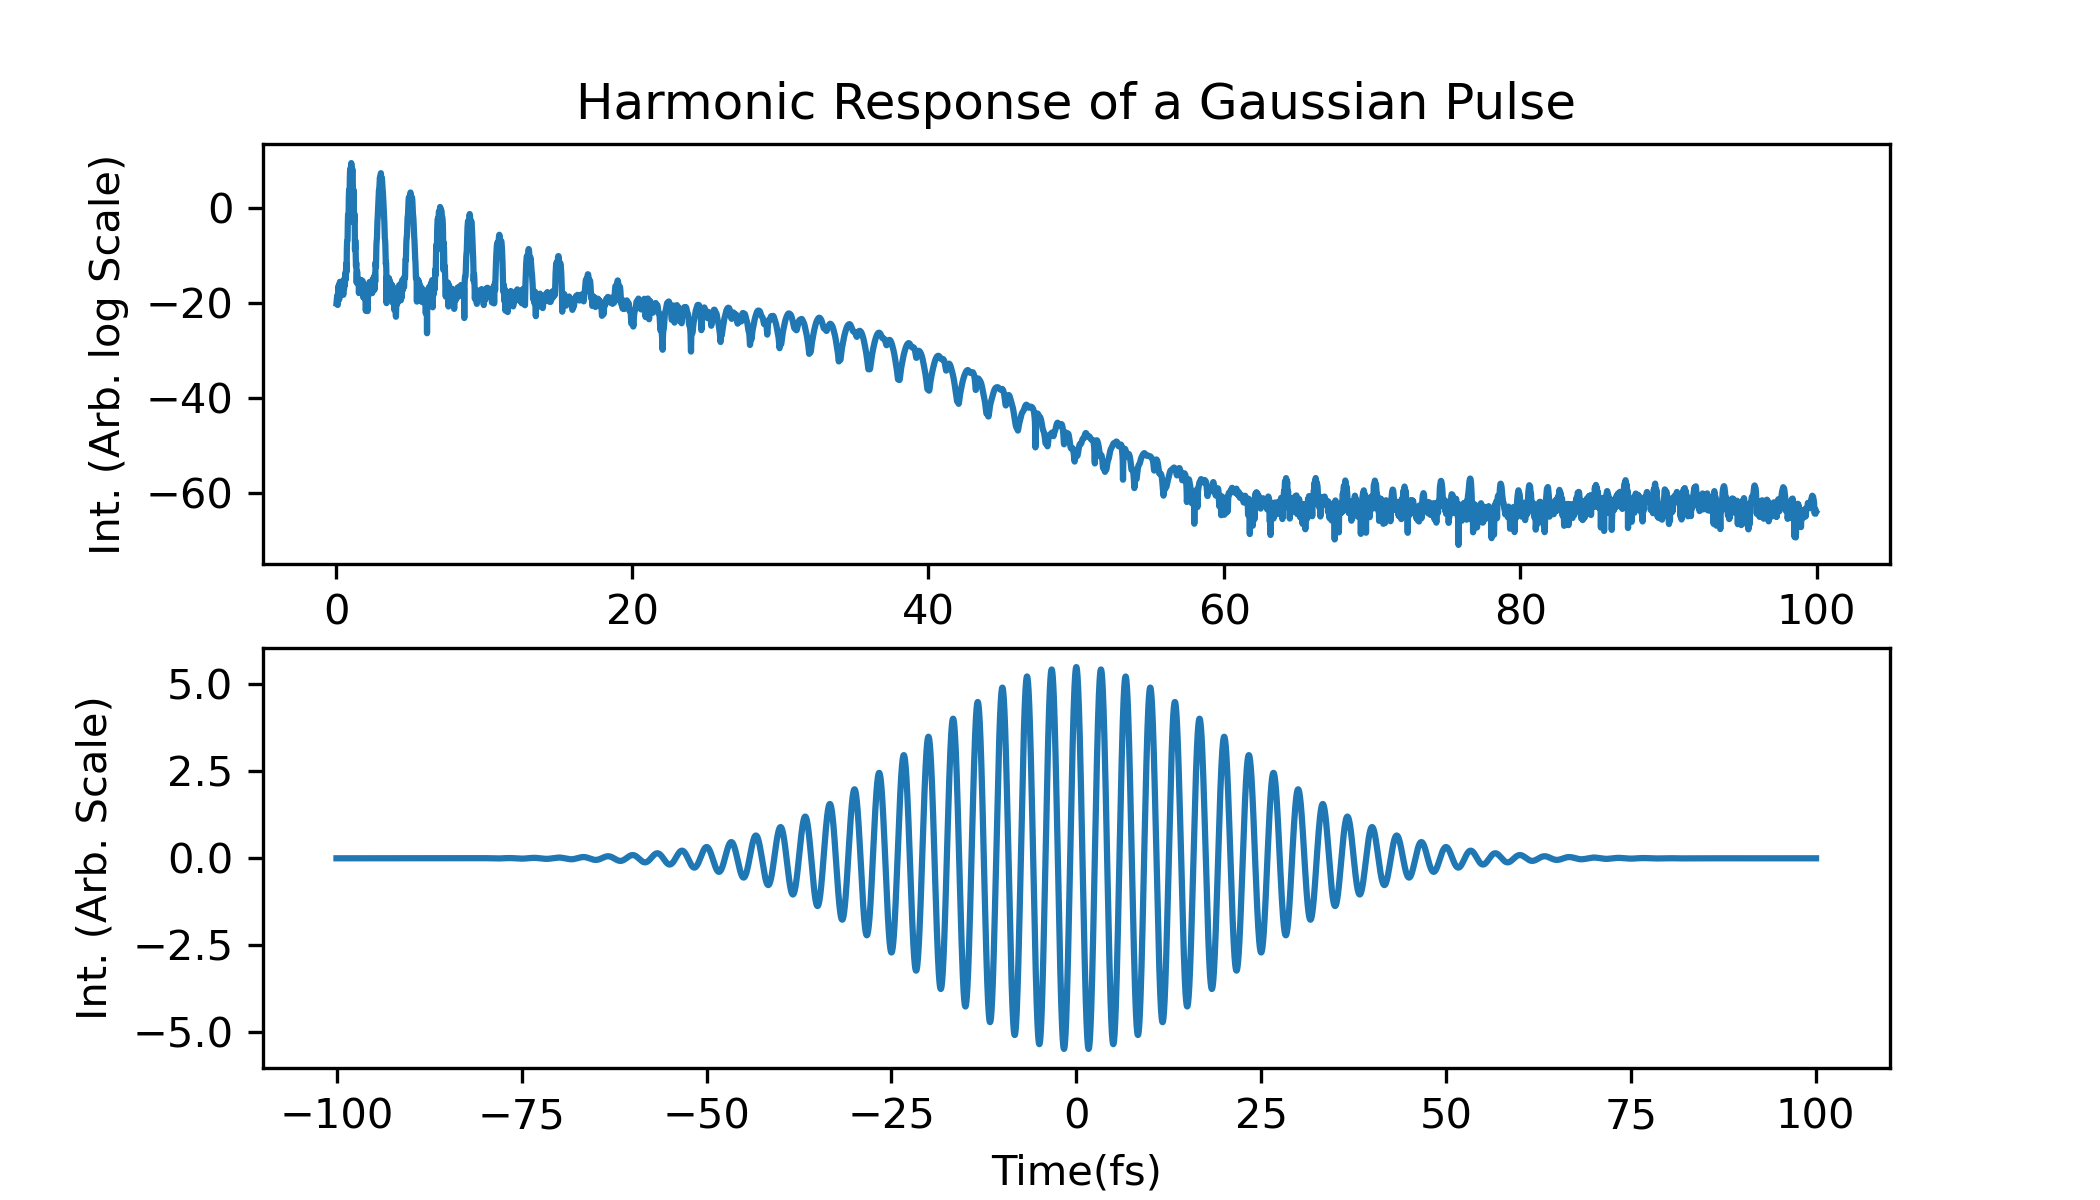
\includegraphics[width=0.8\textwidth]{simpleharmonic.png}
\end{figure}
\newpage

\newgeometry{left=0.14\paperwidth, right=0.14\paperwidth, top=0.06\paperheight, bottom=0.03\paperheight}
\thispagestyle{fancy}
\renewcommand{\headrulewidth}{0pt}
\fancyhead{}
\setlength{\footskip}{0pt}
%

The spectrum looks correct, but in order to ensure the code is accurate, it must follow the cutoff law, where the plateau ends at $E = I_p + 3.17U_p$. To test the cutoff law, we plot the response and draw a line where the cutoff should be, using different pulses:
\begin{figure}[h]
\centering
\includegraphics[width=0.8\textwidth]{cutofflaw.png}
\caption{Plot of harmonic response with increasing intensity and ionization potential, the cutoff is calculated separately and indicated with a vertical line of the same color, verifying the code is functioning properly. The intensity increases by 0.12e14W per line starting at 1e14W for the blue line,ionization potential starts at 12eV and increases by 0.3eV and cutoffs in order from blue to purple are: [33,37,39,43,45] (rounded to the nearest odd integer) }
\end{figure}

One final test we can carry out is to look at the direct output of the response, compared with the input beam:
\begin{figure}[h]
\centering
\includegraphics[width=0.8\textwidth]{directresponse.png}
\end{figure}
\newpage
%\begin{equation}
%\Psi^V_\mathbf{p} (\mathbf{r},t,t') \; = \; \frac{1}{(2\pi)^{3/2}}e^{-iS_V(\mathbf{p},t,t')}  %e^{i[\mathbf{p} + \mathbf{A}(t)]\cdot \mathbf{r}}
%\end{equation}
\newgeometry{left=0.15\paperwidth, right=0.15\paperwidth, top=0.12\paperheight, bottom=0.12\paperheight}
\section{Benchmarking}
After carrying out all of the quick sanity checks, there is only one thing left to see, how fast does it go? To properly carry out a benchmark, every processing run is carried out after a full reboot with no other applications open on the computer and no mouse movement during. Currently, the fastest library for SFA calculations is HHGMax; since SNAIL calculates the same integral, benchmarks will be fair. I will ensure all of the parameters are the same for every run including number of points and integration steps; since HHGMax runs in parallel, I will be using the lewenstein\_parallel module. Each run will include generating the pulse, and a bare call of dipole\_response with no plotting or extra calculations, the loop will be executed in a Matlab script for HHGMax and the results stored, 10 runs are calculated for each point range and the average taken:
\begin{figure}[h]
\centering
\includegraphics[width=0.8\textwidth]{benchmarkplot.png}
\end{figure}
From the graph we can see that both programs scale exponentially, however, SNAIL has a smaller exponential factor. This can be explained by analyzing the code, in the core loop of HHGMax, which is written in C++, there are a number of if statements to check for the unphysical values, these checks are carried out for every single value calculated; in SNAIL, this is automatically handled by the correction array, saving processing time. While C++ loops are far more efficient than Python loops, HHGMax accesses certain arrays in memory every iteration, which is slower than Numpy matrix operations which restrict their pointers. This is slower because HHGMax does not restrict pointers which will never alias; by letting the compiler know that certain variables within your loop will never share the same memory space, it can more aggresively optimize, which is not done here. Additionally, certain variables like dt are declared every iteration, when the code only accepts equally spaced time arrays and could have been declared beforehand. These are all minor things in regular programming, but calculations with large points per cycle and weights can involve tens of millions of iterations or more, so even nanoseconds of difference per loop become noticeable.
\newpage

\section{Final Discussion and Future Work}
During this project, a new library for calculating SFA integral was developed and tested. It agreed closely with the physical theory despite the assumptions of the model, and performed better than the strongest contender in a benchmark; it should provide. 
However, it does not accurately model lower order harmonics, and has a high level of noise in the higher harmonics. The first one is a consequence of the approximations used, whilst there are techniques to reduce noise in Fourier Transforms for the second one. Further simulations are necessary to verify it can reproduce physical effects such as quantum path interference.
\\

The next step will be to write extensive documentation and tests, and publish it as a full software package; while it is currently available online, it lacks automated tests. Afterwards, the next priority will be to develop several color fields, 3D response, and far field propagation. Additionally, \cite{lewensteinog} includes a section on more accurately predicting the lower harmonics, which could be explored. Gabor analysis could also be used to verify the presence of short and long trajectories.
\\

Overall, it should prove a useful tool to quickly get an idea of the results of an experiment or to generate datasets to train neural networks for recognizing patterns in real data; it can also be used to verify the response of novel beam shapes and landscape studies to find new effects. Beyond attosecond physics, with modifications, SNAIL could be used to study the response of molecules, anywhere from $H_2$ to more complicated biomolecules, with the help of more advanced density functional theory packages for the initial state and dipole matrix elements. 

\printbibliography


\end{document}